%!Mode:: "TeX:UTF-8"
%!TEX encoding = UTF-8 Unicode
%lan
%arara: xelatex
\documentclass{ctexart}
\usepackage{amsmath}
\usepackage{tabularray}
\usepackage{amsmath,amssymb}
\usepackage{mathtools}
 \DeclarePairedDelimiter{\norm}{\lVert}{\rVert}
% \DeclarePairedDelimiter{\norm}{\lVert}{\rVert}
\newcommand{\K}{\mathcal{K}}
\newif\ifpreface
%\prefacetrue
\input{../../../global/all}
\begin{document}
\large
\setlength{\baselineskip}{1.2em}
\ifpreface
    \input{../../../global/preface}
\newgeometry{left=2cm,right=2cm,top=2cm,bottom=2cm}
\else
\newgeometry{left=2cm,right=2cm,top=2cm,bottom=2cm}
\maketitle
\fi
%from_here_to_type
% \begin{problem}\label{pro:1}
% \textbf{CGNE:} Solve $A^TAx = A^Tb$.
%
% \begin{align*}
% r_k &= b - Ax_k, \\
% z_k &= A^T r_k, \\
% p_0 &= z_0, \\
% \alpha_k &= \frac{z_k^T z_k}{(Ap_k)^T (Ap_k)}, \\
% x_{k+1} &= x_k + \alpha_k p_k, \\
% r_{k+1} &= r_k - \alpha_k A p_k, \\
% z_{k+1} &= A^T r_{k+1}, \\
% \beta_k &= \frac{z_{k+1}^T z_{k+1}}{z_k^T z_k}, \\
% p_{k+1} &= z_{k+1} + \beta_k p_k.
% \end{align*}
%
% \textbf{CGNR:} Solve $AA^Ty = b$, then $x = A^Ty$.
%
% \begin{align*}
% r_k &= b - AA^T y_k, \\
% p_0 &= r_0, \\
% \alpha_k &= \frac{r_k^T r_k}{(A^T p_k)^T (A^T p_k)}, \\
% y_{k+1} &= y_k + \alpha_k p_k, \\
% r_{k+1} &= r_k - \alpha_k AA^T p_k, \\
% \beta_k &= \frac{r_{k+1}^T r_{k+1}}{r_k^T r_k}, \\
% p_{k+1} &= r_{k+1} + \beta_k p_k.
% \end{align*}
%
% \textbf{BCG:} Two residual sequences:
%
% \begin{align*}
% \alpha_k &= \frac{(r_k, \hat r_k)}{(Ap_k, \hat p_k)}, \\
% x_{k+1} &= x_k + \alpha_k p_k, \\
% r_{k+1} &= r_k - \alpha_k Ap_k, \\
% \hat r_{k+1} &= \hat r_k - \alpha_k A^T \hat p_k, \\
% \beta_k &= \frac{(r_{k+1}, \hat r_{k+1})}{(r_k, \hat r_k)}, \\
% p_{k+1} &= r_{k+1} + \beta_k p_k.
% \end{align*}
% \end{problem}
%
\section{Problem 1}
 \begin{solution}
  
设线性系统为
\[
Ax=b, \qquad r_k=b-Ax_k.
\]
% 若 $A$ 非 Hermitian 或非对称，常见做法是把问题转化为 normal equations，或者使用双共轭梯度类方法。

\subsection*{1. CGNR}
CGNR 的思想是先令
\[
 x=A^*y,
\]
于是原方程变成
\[
AA^*y=b.
\]
对 Hermitian positive definite 矩阵 $AA^*$ 应用 CG。令
\[
r_k=b-AA^*y_k=b-Ax_k, \qquad z_k=A^*r_k.
\]
则 $x_k=A^*y_k$。CGNR 的更新公式可以写为
\[
\alpha_k=\frac{(r_k,r_k)}{(A^*p_k,A^*p_k)},
\]
\[
y_{k+1}=y_k+\alpha_k p_k,
\]
\[
r_{k+1}=r_k-\alpha_k AA^*p_k,
\]
\[
\beta_k=\frac{(r_{k+1},r_{k+1})}{(r_k,r_k)},
\]
\[
p_{k+1}=r_{k+1}+\beta_k p_k.
\]
最后取
\[
x_k=A^*y_k.
\]
也可以直接维护 $x_k$：若 $q_k=A^*p_k$，则
\[
x_{k+1}=x_k+\alpha_k q_k.
\]

\subsection*{2. CGNE}
CGNE 是对
\[
A^*Ax=A^*b
\]
应用 CG。令
\[
r_k=b-Ax_k, \qquad z_k=A^*r_k.
\]
其中 $z_k$ 是 normal equation 的 residual。取初值
\[
z_0=A^*r_0, \qquad p_0=z_0.
\]
更新公式为
\[
\alpha_k=\frac{(z_k,z_k)}{(Ap_k,Ap_k)},
\]
\[
x_{k+1}=x_k+\alpha_k p_k,
\]
\[
r_{k+1}=r_k-\alpha_k Ap_k,
\]
\[
z_{k+1}=A^*r_{k+1},
\]
\[
\beta_k=\frac{(z_{k+1},z_{k+1})}{(z_k,z_k)},
\]
\[
p_{k+1}=z_{k+1}+\beta_kp_k.
\]
因此 CGNE 的 Krylov 子空间为
\[
x_k\in x_0+\K_k(A^*A,A^*r_0).
\]

\subsection*{3. BCG}
BCG，即 Bi-Conjugate Gradient，同时构造两个 residual 序列 $r_k$ 和 $\hat r_k$，分别对应 $A$ 和 $A^*$。给定 $x_0$，令
\[
r_0=b-Ax_0,
\]
并选择 $\hat r_0$ 使得
\[
(\hat r_0,r_0)\ne 0.
\]
通常取 $\hat r_0=r_0$。设
\[
p_0=r_0, \qquad \hat p_0=\hat r_0.
\]
BCG 的更新为
\[
\alpha_k=\frac{(\hat r_k,r_k)}{(\hat p_k,Ap_k)},
\]
\[
x_{k+1}=x_k+\alpha_kp_k,
\]
\[
r_{k+1}=r_k-\alpha_kAp_k,
\]
\[
\hat r_{k+1}=\hat r_k-\overline{\alpha_k}A^*\hat p_k,
\]
\[
\beta_k=\frac{(\hat r_{k+1},r_{k+1})}{(\hat r_k,r_k)},
\]
\[
p_{k+1}=r_{k+1}+\beta_kp_k,
\]
\[
\hat p_{k+1}=\hat r_{k+1}+\overline{\beta_k}\hat p_k.
\]
BCG 的核心正交关系为
\[
(\hat r_i,r_j)=0, \qquad i\ne j,
\]
以及双共轭关系
\[
(\hat p_i,Ap_j)=0, \qquad i\ne j.
\]

\end{solution}
\section{Problem 2}
\begin{solution}
   设 $A$ 是 unitary shift matrix，$b=e_1$，$x_0=0$。因为 $A$ 是 unitary 矩阵，所以
\[
A^*A=I.
\]
CGNE 对 normal equation
\[
A^*Ax=A^*b
\]
应用 CG，因此该方程变成
\[
x=A^*b.
\]
所以 CGNE 一步收敛。

对于 GMRES，$A$ 是 $n\times n$ cyclic shift matrix，则它的 minimal polynomial 为
\[
m_A(z)=z^n-1.
\]
从零初值出发，GMRES 的 residual 可以写成
\[
r_k=p_k(A)r_0, \qquad p_k(0)=1,\quad \deg(p_k)\le k.
\]
若 $k<n$，不存在次数小于 $n$ 且满足 $p(A)e_1=0$ 的 admissible polynomial。
      因此 GMRES 通常需要 $n$ 步才能精确解出。

CGS 是基于 BiCG residual polynomial 的平方，其收敛同样受 minimal polynomial 控制。
      由于该问题中要消去 cyclic shift 结构至少需要 $n$ 阶信息，
      因此 CGS 至少需要与 $n$ 同阶的 matrix-vector multiplications。
      由于 CGS 每步通常需要两次 $A$ 的乘法，因此可给出下界：需要 $O(n)$ 次 matrix-vector multiplications。

结论：
\[
\text{CGNE: 1 step}, \qquad \text{GMRES: } n \text{ steps}, \qquad \text{CGS: at least order } n \text{ matvecs}.
\]

\subsection*{(b) CGNE loses}
设
\[
A=\operatorname{diag}(M_1,M_2,\ldots,M_{n/2}),
\]
其中
\[
M_j=\begin{pmatrix}1&j-1\\0&1\end{pmatrix}.
\]
每个 $M_j$ 都可以写成
\[
M_j=I+N_j,
\]
其中
\[
N_j=\begin{pmatrix}0&j-1\\0&0\end{pmatrix}, \qquad N_j^2=0.
\]
因此
\[
(M_j-I)^2=0.
\]
若存在某个 $j>1$，则 $M_j\ne I$，所以 $M_j-I\ne 0$。因此整个矩阵 $A$ 的 minimal polynomial 为
\[
m_A(z)=(z-1)^2.
\]
GMRES 方法产生的残差可以表示为
\[
r_k = p_k(A) r_0,
\]
其中 $p_k$ 是次数不超过 $k$ 的多项式，并满足 $p_k(0)=1$。

由于矩阵 $A$ 的最小多项式为
\[
m_A(z) = (z-1)^2,
\]
因此有
\[
m_A(A) = 0。
\]

当迭代步数 $k=2$ 时，GMRES 可以选取一个次数不超过 $2$ 的多项式。特别地，可以取
\[
p_2(z) = (z-1)^2。
\]
于是有
\[
r_2 = p_2(A) r_0 = m_A(A) r_0 = 0。
\]

因此，GMRES 在至多 $2$ 步内可以得到精确解。

对于 CGS，如果 $\hat r_0=r_0$ 且不发生 breakdown，则它的 residual polynomial 是 BiCG residual polynomial 的平方。因为 minimal polynomial 的次数为 $2$，所以 CGS 也会在很少步内收敛，通常需要约 $2$ 步；考虑到 CGS 每步需要两次 matrix-vector multiplication，因此约需要 $4$ 次 matrix-vector multiplications。

但是 CGNE 应用于
\[
A^*Ax=A^*b.
\]
题目给出该矩阵的 singular values 大约分布在
\[
[2/n,n/2].
\]
所以
\[
\kappa(A)\approx \frac{n/2}{2/n}=\frac{n^2}{4}.
\]
而 CGNE 实际面对的是 $A^*A$，其条件数为
\[
\kappa(A^*A)=\kappa(A)^2\approx \frac{n^4}{16}.
\]
当 $n$ 很大时，条件数极大，因此 CGNE 会需要很多迭代。

\subsection*{(c) CGS wins}
该问题中矩阵 $A$ 为 Hermitian，且其特征值分布在正实区间 $[c,d]$ 上。

首先考虑 CGNE 方法。该方法等价于对正规方程 $A^TAx=A^Tb$ 应用共轭梯度法。
由于 $A$ 为 Hermitian，其特征值为实数且非负，因此
\[
\kappa(A^TA) = \frac{\lambda_{\max}(A^TA)}{\lambda_{\min}(A^TA)}
= \frac{\lambda_{\max}(A)^2}{\lambda_{\min}(A)^2}
= \kappa(A)^2。
\]
而共轭梯度法的收敛速度满足
\[
\frac{\norm*{r_k}}{\norm*{r_0}} 
\le 2\left(\frac{\sqrt{\kappa}-1}{\sqrt{\kappa}+1}\right)^k，
\]
因此当条件数平方后，收敛速度显著变慢，需要更多迭代次数，
从而导致总计算量较大。

其次考虑 GMRES 方法。GMRES 在第 $k$ 步产生的残差满足
\[
\norm*{r_k} 
= \min_{p_k \in \mathcal{P}_k,\, p_k(0)=1} \norm*{p_k(A)r_0}。
\]
当特征值分布在整个区间 $[c,d]$ 上时，很难用低次数多项式在整个区间上同时逼近零，
因此需要较大的 $k$ 才能显著降低残差。此外，GMRES 每一步需要进行 Arnoldi 正交化，
其计算成本约为 $O(k^2 n)$，因此总体计算量较大。

最后考虑 CGS 方法。CGS 来源于 BiCG 方法的平方形式，
在 Hermitian 情形下，BiCG 与共轭梯度法具有密切关系，
其搜索方向与 CG 方法生成的 Krylov 子空间一致。
因此 CGS 的收敛行为在一定程度上类似于 CG 方法，
能够利用特征值分布信息实现较快收敛。

同时，CGS 每一步只涉及有限次矩阵-向量乘法，
且不需要像 GMRES 那样进行正交化操作，
因此单步计算成本较低。

综上，在 GMRES、CGS 和 CGNE 三种方法中，
CGS 通常需要最少的计算量（flops）。
\subsection*{(d) CGS loses}
设
\[
A=\begin{pmatrix}0&1\\-1&0\end{pmatrix}\otimes I_{n/2}.
\]
每个 $2\times2$ block 记为
\[
J=\begin{pmatrix}0&1\\-1&0\end{pmatrix}.
\]
有
\[
J^T=-J, \qquad J^TJ=I.
\]
因此
\[
A^TA=I, \qquad AA^T=I.
\]
所以 $A$ 是 normal matrix。又因为
\[
J^2=-I,
\]
故 $J$ 的 eigenvalues 为
\[
\lambda=\pm i.
\]
因此 $A$ 的 eigenvalues 也为 $\pm i$，singular values 全部为 $1$。

CGNE 对
\[
A^TAx=A^Tb
\]
应用 CG。由于 $A^TA=I$，所以 CGNE 一步收敛。

GMRES 的 minimal polynomial 为
\[
m_A(z)=z^2+1.
\]
因此 GMRES 至多需要 $2$ 步。

下面说明 CGS 会 breakdown。CGS 中若取 $\hat r_0=r_0$，第一步的分母含有
\[
(\hat r_0,Ar_0)=(r_0,Ar_0).
\]
由于 $A^T=-A$，对任意实向量 $r_0$，有
\[
(r_0,Ar_0)=r_0^TAr_0.
\]
而
\[
(r_0^TAr_0)^T=r_0^TA^Tr_0=-r_0^TAr_0.
\]
所以
\[
r_0^TAr_0=0.
\]
因此第一步更新中的分母为 $0$，CGS 在第一步发生 breakdown。


\end{solution}

\section*{Problem 3}
\begin{solution}

设
\[
A=I-F, \qquad F=-F^*.
\]
因此 $F$ 是 skew-Hermitian，$A$ 的 eigenvalues 位于线段
\[
[1-i\gamma,1+i\gamma].
\]
题目给出的 MINRES residual bound 为
\[
\frac{\norm{r_n}}{\norm{r_0}}\le \frac{2}{R^n+R^{-n}},
\qquad
R=\frac{1+\sqrt{1+\gamma^2}}{\gamma}.
\]

CGNR 对
\[
AA^*y=b, \qquad x=A^*y
\]
应用 CG。若 $A$ 的 eigenvalues 为
\[
\lambda=1+i t, \qquad t\in[-\gamma,\gamma],
\]
则 $AA^*$ 的 eigenvalues 为
\[
|\lambda|^2=1+t^2.
\]
因此
\[
\lambda(AA^*)\subset [1,1+\gamma^2].
\]
所以
\[
\kappa(AA^*)=1+\gamma^2.
\]
CG 的经典误差界给出
\[
\frac{\norm{r_n^{\rm CGNR}}}{\norm{r_0}}
\le
2\left(\frac{\sqrt{1+\gamma^2}-1}{\sqrt{1+\gamma^2}+1}\right)^n.
\]
令
\[
\rho_{\rm CGNR}=\frac{\sqrt{1+\gamma^2}-1}{\sqrt{1+\gamma^2}+1}.
\]
另一方面，MINRES 的界中
\[
R=\frac{1+\sqrt{1+\gamma^2}}{\gamma}.
\]
可以验证
\[
R^{-2}=\frac{\sqrt{1+\gamma^2}-1}{\sqrt{1+\gamma^2}+1}=\rho_{\rm CGNR}.
\]
因此 CGNR 的收敛因子大约为 $R^{-2n}$，而 MINRES 的界大约为 $R^{-n}$。这说明从这个理论界看，CGNR 可能比 MINRES 更快一个平方因子。

但是需要注意：CGNR 每一步涉及 $A$ 和 $A^*$ 的乘法，而且它作用在 normal equation 上，可能会放大条件数和舍入误差。因此就实际计算成本和稳定性而言，不能简单地说 CGNR 一定优于 MINRES。若只比较 residual bound 的指数衰减，CGNR 的界更快；若比较每步代价与数值稳定性，MINRES 通常更自然。

\end{solution}

\section{Problem 4}
\begin{solution}
设 $\{q_{n+1}\}$ 是在区间 $[-1,1]$ 上关于正权函数 $w(x)>0$ 的正交多项式序列。
假设 $q_{n+1}$ 是次数为 $n$ 的多项式。我们证明 $q_{n+1}$ 在 $(-1,1)$ 内有 $n$ 个互异零点。

由正交性，对任意次数不超过 $n-1$ 的多项式 $p(x)$，都有
\[
\int_{-1}^1 q_{n+1}(x)p(x)w(x)\,dx=0.
\]

设 $q_{n+1}$ 在 $(-1,1)$ 内所有奇数重数的零点为
\[
x_1,x_2,\ldots,x_m.
\]
如果 $m<n$，取
\[
p(x)=\prod_{j=1}^m (x-x_j).
\]
则
\[
\deg p=m<n,
\]
所以 $p\in \mathbb{P}_{n-1}$。

注意到 $q_{n+1}$ 只有在奇数重数零点处才会改变符号，而 $p(x)$ 也恰好在每个
$x_j$ 处改变符号。因此乘积 $q_{n+1}(x)p(x)$ 在整个区间 $(-1,1)$ 上符号不变。
并且 $q_{n+1}(x)p(x)$ 不是零多项式，所以它在某个子区间上严格同号。

由于 $w(x)>0$，因此
\[
\int_{-1}^1 q_{n+1}(x)p(x)w(x)\,dx \ne 0.
\]
这与正交性矛盾。

因此必须有
\[
m\ge n.
\]
也就是说，$q_{n+1}$ 在 $(-1,1)$ 内至少有 $n$ 个奇数重数零点。

另一方面，$q_{n+1}$ 是次数为 $n$ 的多项式，所以它最多只有 $n$ 个零点，按重数计算也不超过 $n$。
因此 $q_{n+1}$ 在 $(-1,1)$ 内恰好有 $n$ 个零点，而且每个零点的重数都只能是 $1$。
否则，若某个零点重数大于 $1$，按重数计算零点个数就会超过 $n$。

故 $q_{n+1}$ 在 $(-1,1)$ 内有 $n$ 个互异零点。

因此，
\[
q_{n+1} \text{ has } n \text{ distinct zeros in } (-1,1).
\]

\end{solution}

\section*{Problem 5}
\begin{solution}
  

给定 $n$ 个互异节点
\[
x_1,x_2,\ldots,x_n\in[-1,1].
\]
要求求积公式
\[
I_n(f)=\sum_{j=1}^n w_j f(x_j)
\]
对所有次数不超过 $n-1$ 的多项式精确，即
\[
\int_{-1}^1 p(x)\,dx=\sum_{j=1}^n w_jp(x_j),
\qquad \forall p\in\mathbb{P}_{n-1}.
\]

令 $\ell_j(x)$ 是 Lagrange 基函数：
\[
\ell_j(x)=\prod_{i\ne j}\frac{x-x_i}{x_j-x_i}.
\]
则
\[
\ell_j(x_i)=\delta_{ij}.
\]
对任意 $p\in\mathbb{P}_{n-1}$，有插值表示
\[
p(x)=\sum_{j=1}^n p(x_j)\ell_j(x).
\]
两边积分得
\[
\int_{-1}^1 p(x)\,dx
=
\sum_{j=1}^n p(x_j)\int_{-1}^1\ell_j(x)\,dx.
\]
因此只要取
\[
w_j=\int_{-1}^1\ell_j(x)\,dx,
\]
求积公式就对所有 $\deg p\le n-1$ 的多项式精确。

下面证明唯一性。若还有另一组权重 $\{\tilde w_j\}$ 也满足精确性，则对 $p=\ell_k$，有
\[
\int_{-1}^1\ell_k(x)\,dx
=
\sum_{j=1}^n \tilde w_j\ell_k(x_j)
=
\tilde w_k.
\]
因此
\[
\tilde w_k=w_k,
\qquad k=1,2,\ldots,n.
\]
所以权重唯一。

\end{solution}

\section*{Problem 6}
\begin{solution}
% \subsection{(a) 方法说明}

本题采用 Golub--Welsch 算法计算 $n$ 点 Gauss--Legendre 求积公式的节点和权重。
构造 Jacobi 矩阵
\[
J = \begin{pmatrix}
0 & \beta_1 &  &  \\
\beta_1 & 0 & \ddots &  \\
 & \ddots & \ddots & \beta_{n-1} \\
 &  & \beta_{n-1} & 0
\end{pmatrix},
\quad
\beta_k = \frac{k}{\sqrt{4k^2-1}}。
\]
矩阵 $J$ 的特征值即为求积节点 $x_i$，对应特征向量第一分量的平方给出权重：
\[
w_i = 2 (v_{1i})^2。
\]

\subsection{(b) 函数 $f(x)=e^x$}

精确积分为
\[
I(f)=\int_{-1}^1 e^x\,dx = e^1 - e^{-1}。
\]

计算误差
\[
|I(f)-I_n(f)| = \left| \int_{-1}^1 e^x\,dx - \sum_{i=1}^n w_i e^{x_i} \right|。
\]

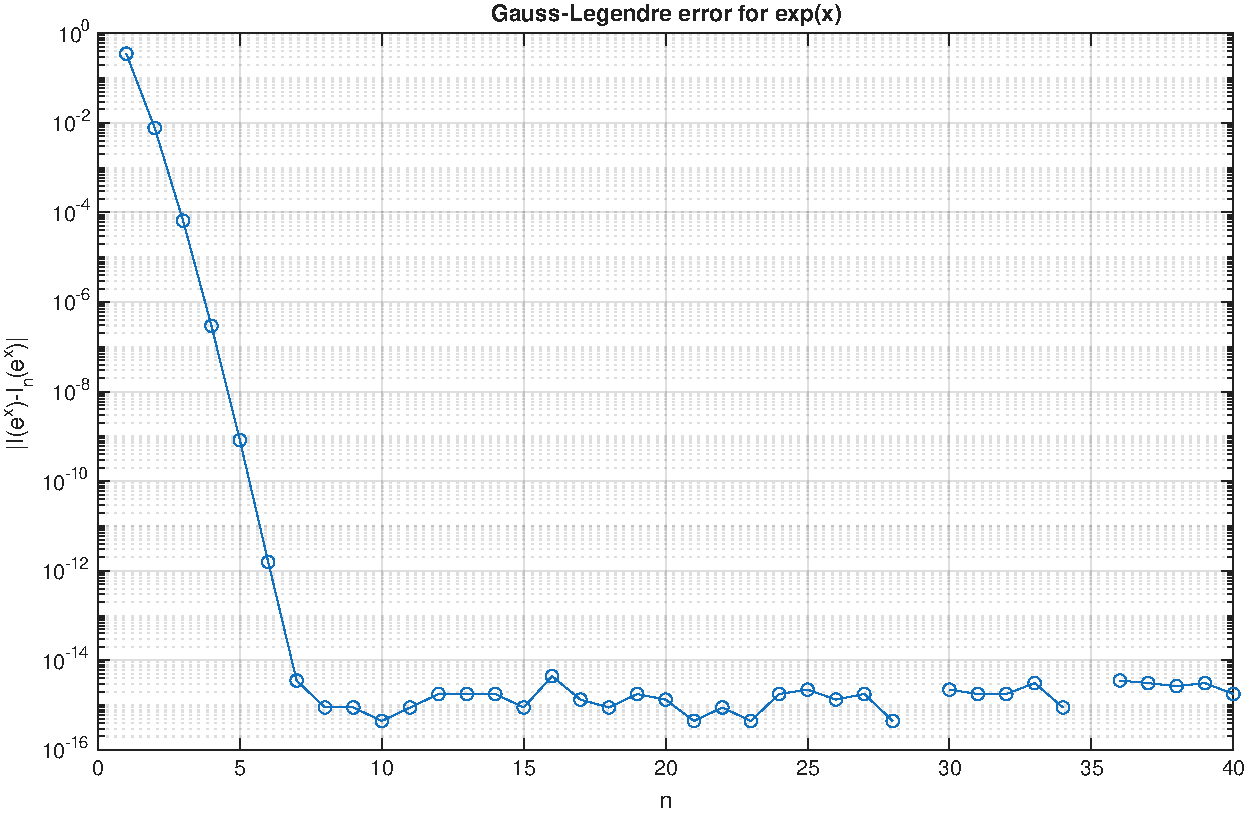
\includegraphics[width=\textwidth]{exp_error.pdf}
数值结果（对数坐标下）表明，随着 $n$ 的增加，误差迅速下降，呈现近似指数收敛。
这一现象可以从理论上解释：函数 $f(x)=e^x$ 在区间 $[-1,1]$ 上是解析函数，
可以被高精度的多项式很好地逼近。而 Gauss--Legendre 求积公式对次数不超过
$2n-1$ 的多项式是精确的，因此对于解析函数，其误差会随 $n$ 指数级下降。

\subsection*{(c) 函数 $f(x)=e^{|x|}$}

精确积分为
\[
I(f)=\int_{-1}^1 e^{|x|}\,dx = 2(e^1-1)。
\]

同样计算误差
\[
|I(f)-I_n(f)|。
\]
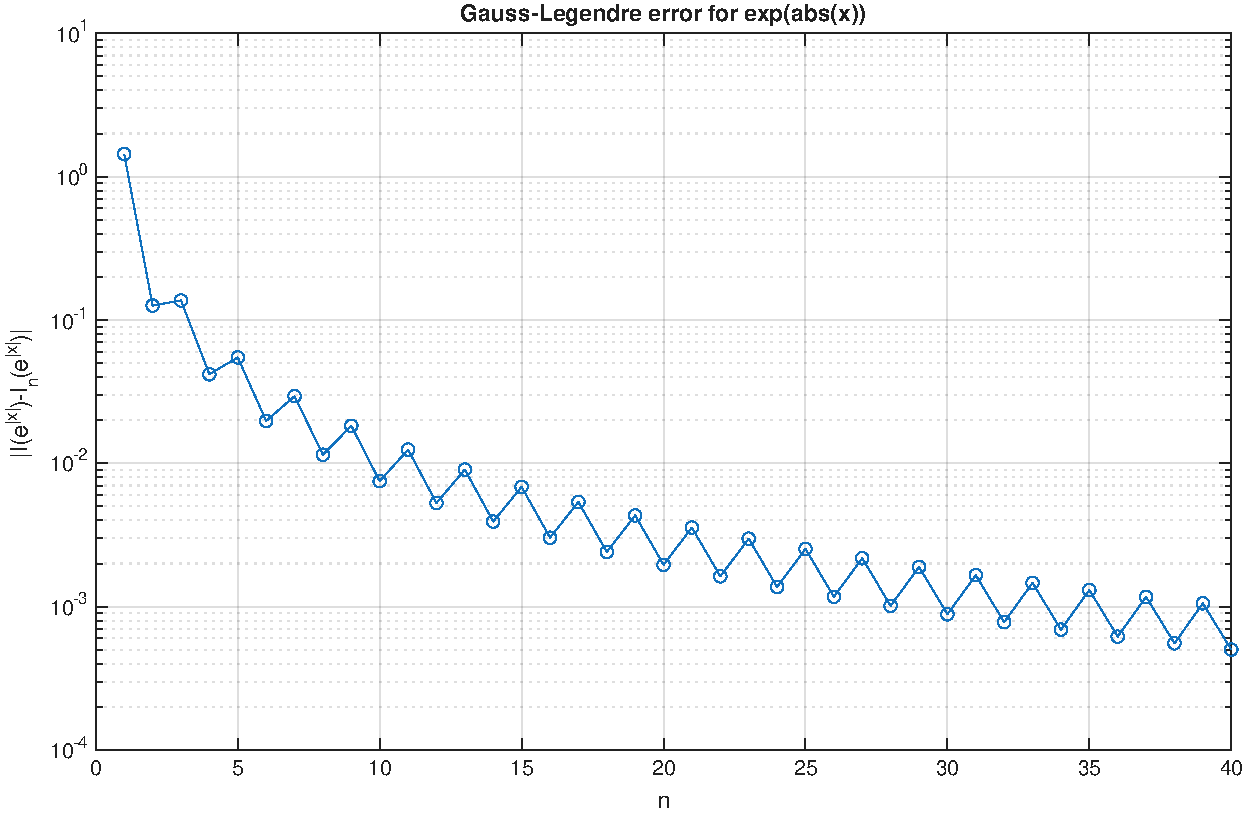
\includegraphics[width=\textwidth]{ exp_abs_error.pdf}
数值结果表明，误差仍然随 $n$ 增加而减小，但收敛速度明显慢于 $f(x)=e^x$ 的情况。

这是因为函数 $f(x)=e^{|x|}$ 在 $x=0$ 处不可导（存在尖点），不再是光滑函数。
函数的非光滑性会显著降低多项式逼近的效果，从而使得 Gauss--Legendre
求积的收敛速度从指数级降低为代数级。


实验表明，Gauss--Legendre 求积公式的收敛速度与被积函数的光滑性密切相关。
对于解析函数，可以获得指数收敛；而对于存在不可导点的函数，收敛速度显著降低。
\end{solution}
\section*{Problem 7}
\begin{solution}

构造
\[
A=U\Sigma V,
\]
其中 $U,V$ 是随机正交矩阵，
\[
\Sigma=\operatorname{diag}(\sigma_1,\ldots,\sigma_m),
\]
并且
\[
\sigma_i=\kappa^{\frac{i-1}{m-1}},
\qquad i=1,2,\ldots,m,
\]
其中
\[
\kappa=10^4,
\qquad m=40.
\]
注意若希望 singular values 从大到小排列，也可以使用
\[
\sigma_i=\kappa^{-\frac{i-1}{m-1}}.
\]
这只改变尺度排序，不改变条件数。


\begin{figure}[h]
\centering
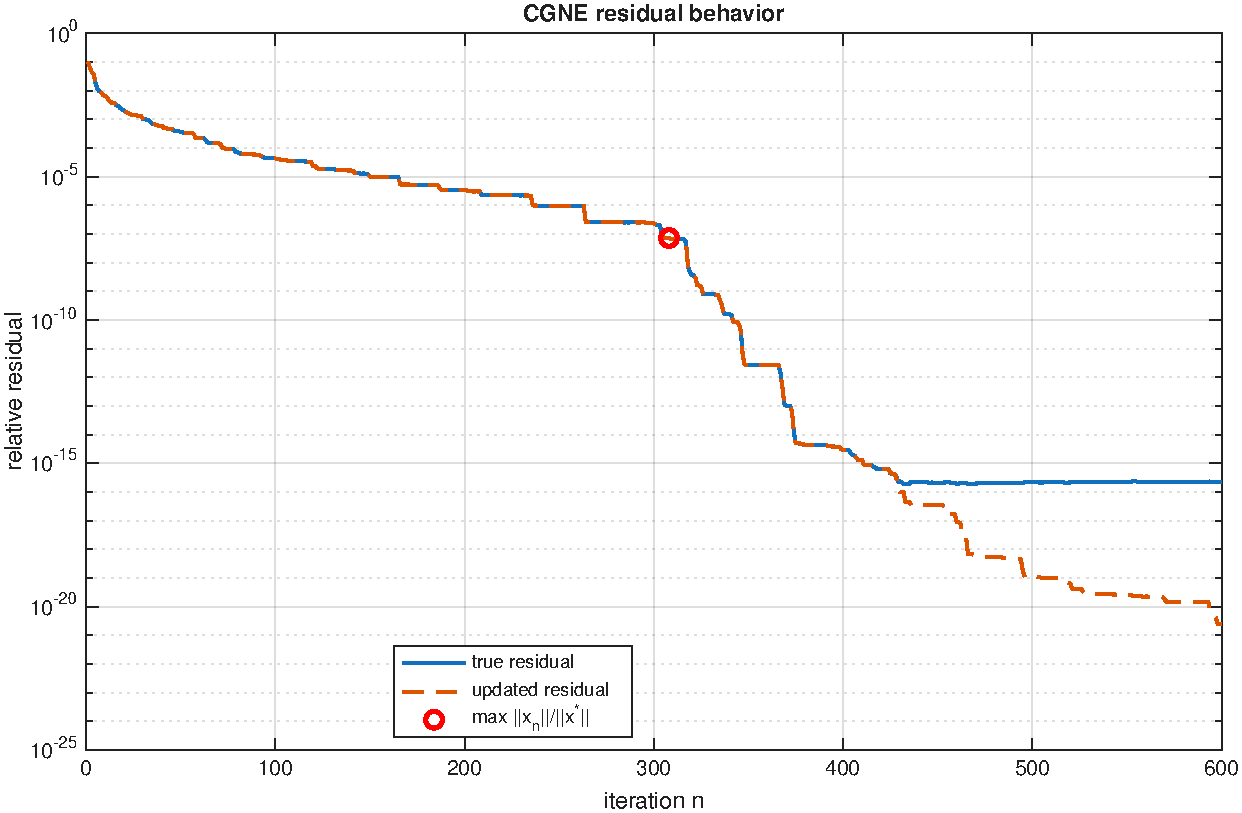
\includegraphics[width=0.7\textwidth]{cgne_residual.pdf}
\caption{CGNE 方法的残差行为：真实残差与递推残差的对比，以及 $\max \norm{x_k}/\norm{x^*}$ 的位置。}
\label{fig:cgne}
\end{figure}
\end{solution}
\section*{Problem 8}
\begin{solution}


下面比较 CG、GMRES、CGN 和 BCG。这里 CGN 指 CGNE/CGNR 一类 normal equation 方法。

\begin{enumerate}

\item 

最优方法：GMRES。

理由：GMRES 在第 $k$ 步的残差满足
\[
\norm*{r_k} = \min_{p_k \in \mathcal{P}_k,\; p_k(0)=1} \norm*{p_k(A)r_0}.
\]
当特征值高度聚集在 $-1$ 附近时，可以构造低次数多项式 $p_k$，
使其在该聚集区域上迅速衰减，从而在较少迭代步内显著降低残差。
由于矩阵是稠密的，每次矩阵-向量乘法代价较高，因此减少迭代次数尤为重要，
GMRES 在此情形下具有明显优势。

\item 

最优方法：GMRES 或 BCG。

理由：当特征值在复平面中广泛分布时，很难用低次数多项式在整个谱上同时逼近零，
因此 GMRES 可能需要较多迭代步。此外，GMRES 每步需要进行 Arnoldi 正交化，
计算成本约为 $O(k^2 n)$，存储成本也随 $k$ 增长。

BCG 采用短递推，每步计算成本为常数量级的矩阵-向量乘法，
因此在大规模问题中更具计算优势。但其数值稳定性较差，
可能出现 breakdown 或收敛不稳定。CGN 方法由于求解 $A^TAx=A^Tb$，
会导致条件数平方，从而进一步减慢收敛速度，因此通常不是优选。

\item 

最优方法：BCG 或重启 GMRES。

理由：对于如此大规模问题，完全 GMRES 的存储需求为 $O(km)$，
在实际中不可行。由于特征值聚集，理论上存在低次数多项式可以快速衰减误差，
因此 Krylov 方法收敛较快。

BCG 具有短递推结构，仅需存储有限个向量，适合大规模稀疏问题。
重启 GMRES 可以限制存储成本，但可能影响收敛速度，是一种折中方案。

\item 

最优方法：CG。

理由：矩阵为 Hermitian 正定，其特征值为实且正。
CG 方法在该情形下具有最优性质，其误差满足
\[
\frac{\norm*{e_k}}{\norm*{e_0}} \le 
2\left(\frac{\sqrt{\kappa}-1}{\sqrt{\kappa}+1}\right)^k,
\]
其中 $\kappa = \frac{\lambda_{\max}}{\lambda_{\min}}$。
由于条件数适中，CG 能以较少迭代达到高精度，
且每步仅需一次矩阵-向量乘法和少量内积运算，计算效率高。

\item 

最优方法：CG。

理由：矩阵仍为 Hermitian 正定，因此 CG 仍适用。
离群特征值会增大条件数，从而降低收敛速度，
但 CG 的收敛过程可以看作在 Krylov 子空间中逐步消除不同特征方向的误差，
通常可以较快地抑制主导特征值方向的误差。
在实际应用中，可通过预条件化改善该问题。

\item 

最优方法：GMRES（或 MINRES；在给定方法中选 GMRES）。

理由：此时矩阵为 Hermitian 但不再正定，CG 方法不再适用。
GMRES 对一般矩阵具有良好的鲁棒性，适用于不定问题。
BCG 虽然可用，但存在 breakdown 风险。
CGN 方法通过构造 $A^TA$ 会丢失原矩阵的符号信息，
并将谱平方，从而可能导致更差的数值性质。

\item 

最优方法：GMRES。

理由：对于正规矩阵（$AA^*=A^*A$），其谱性质可以很好地描述收敛行为。
GMRES 的误差由多项式在谱上的最大值控制，
而在环形区域上可以构造合适的多项式实现较好的收敛。
CG 方法不适用于一般非 Hermitian 问题，
CGN 会引入条件数平方效应，BCG 则稳定性较差。

\end{enumerate}
\end{solution}

\end{document}
